\documentclass[1p]{elsarticle_modified}
%\bibliographystyle{elsarticle-num}

%\usepackage[colorlinks]{hyperref}
%\usepackage{abbrmath_seonhwa} %\Abb, \Ascr, \Acal ,\Abf, \Afrak
\usepackage{amsfonts}
\usepackage{amssymb}
\usepackage{amsmath}
\usepackage{amsthm}
\usepackage{scalefnt}
\usepackage{amsbsy}
\usepackage{kotex}
\usepackage{caption}
\usepackage{subfig}
\usepackage{color}
\usepackage{graphicx}
\usepackage{xcolor} %% white, black, red, green, blue, cyan, magenta, yellow
\usepackage{float}
\usepackage{setspace}
\usepackage{hyperref}

\usepackage{tikz}
\usetikzlibrary{arrows}

\usepackage{multirow}
\usepackage{array} % fixed length table
\usepackage{hhline}

%%%%%%%%%%%%%%%%%%%%%
\makeatletter
\renewcommand*\env@matrix[1][\arraystretch]{%
	\edef\arraystretch{#1}%
	\hskip -\arraycolsep
	\let\@ifnextchar\new@ifnextchar
	\array{*\c@MaxMatrixCols c}}
\makeatother %https://tex.stackexchange.com/questions/14071/how-can-i-increase-the-line-spacing-in-a-matrix
%%%%%%%%%%%%%%%

\usepackage[normalem]{ulem}

\newcommand{\msout}[1]{\ifmmode\text{\sout{\ensuremath{#1}}}\else\sout{#1}\fi}
%SOURCE: \msout is \stkout macro in https://tex.stackexchange.com/questions/20609/strikeout-in-math-mode

\newcommand{\cancel}[1]{
	\ifmmode
	{\color{red}\msout{#1}}
	\else
	{\color{red}\sout{#1}}
	\fi
}

\newcommand{\add}[1]{
	{\color{blue}\uwave{#1}}
}

\newcommand{\replace}[2]{
	\ifmmode
	{\color{red}\msout{#1}}{\color{blue}\uwave{#2}}
	\else
	{\color{red}\sout{#1}}{\color{blue}\uwave{#2}}
	\fi
}

\newcommand{\Sol}{\mathcal{S}} %segment
\newcommand{\D}{D} %diagram
\newcommand{\A}{\mathcal{A}} %arc


%%%%%%%%%%%%%%%%%%%%%%%%%%%%%5 test

\def\sl{\operatorname{\textup{SL}}(2,\Cbb)}
\def\psl{\operatorname{\textup{PSL}}(2,\Cbb)}
\def\quan{\mkern 1mu \triangleright \mkern 1mu}

\theoremstyle{definition}
\newtheorem{thm}{Theorem}[section]
\newtheorem{prop}[thm]{Proposition}
\newtheorem{lem}[thm]{Lemma}
\newtheorem{ques}[thm]{Question}
\newtheorem{cor}[thm]{Corollary}
\newtheorem{defn}[thm]{Definition}
\newtheorem{exam}[thm]{Example}
\newtheorem{rmk}[thm]{Remark}
\newtheorem{alg}[thm]{Algorithm}

\newcommand{\I}{\sqrt{-1}}
\begin{document}

%\begin{frontmatter}
%
%\title{Boundary parabolic representations of knots up to 8 crossings}
%
%%% Group authors per affiliation:
%\author{Yunhi Cho} 
%\address{Department of Mathematics, University of Seoul, Seoul, Korea}
%\ead{yhcho@uos.ac.kr}
%
%
%\author{Seonhwa Kim} %\fnref{s_kim}}
%\address{Center for Geometry and Physics, Institute for Basic Science, Pohang, 37673, Korea}
%\ead{ryeona17@ibs.re.kr}
%
%\author{Hyuk Kim}
%\address{Department of Mathematical Sciences, Seoul National University, Seoul 08826, Korea}
%\ead{hyukkim@snu.ac.kr}
%
%\author{Seokbeom Yoon}
%\address{Department of Mathematical Sciences, Seoul National University, Seoul, 08826,  Korea}
%\ead{sbyoon15@snu.ac.kr}
%
%\begin{abstract}
%We find all boundary parabolic representation of knots up to 8 crossings.
%
%\end{abstract}
%\begin{keyword}
%    \MSC[2010] 57M25 
%\end{keyword}
%
%\end{frontmatter}

%\linenumbers
%\tableofcontents
%
\newcommand\colored[1]{\textcolor{white}{\rule[-0.35ex]{0.8em}{1.4ex}}\kern-0.8em\color{red} #1}%
%\newcommand\colored[1]{\textcolor{white}{ #1}\kern-2.17ex	\textcolor{white}{ #1}\kern-1.81ex	\textcolor{white}{ #1}\kern-2.15ex\color{red}#1	}

{\Large $\underline{11n_{95}~(K11n_{95})}$}

\setlength{\tabcolsep}{10pt}
\renewcommand{\arraystretch}{1.6}
\vspace{1cm}\begin{tabular}{m{100pt}>{\centering\arraybackslash}m{274pt}}
\multirow{5}{120pt}{
	\centering
	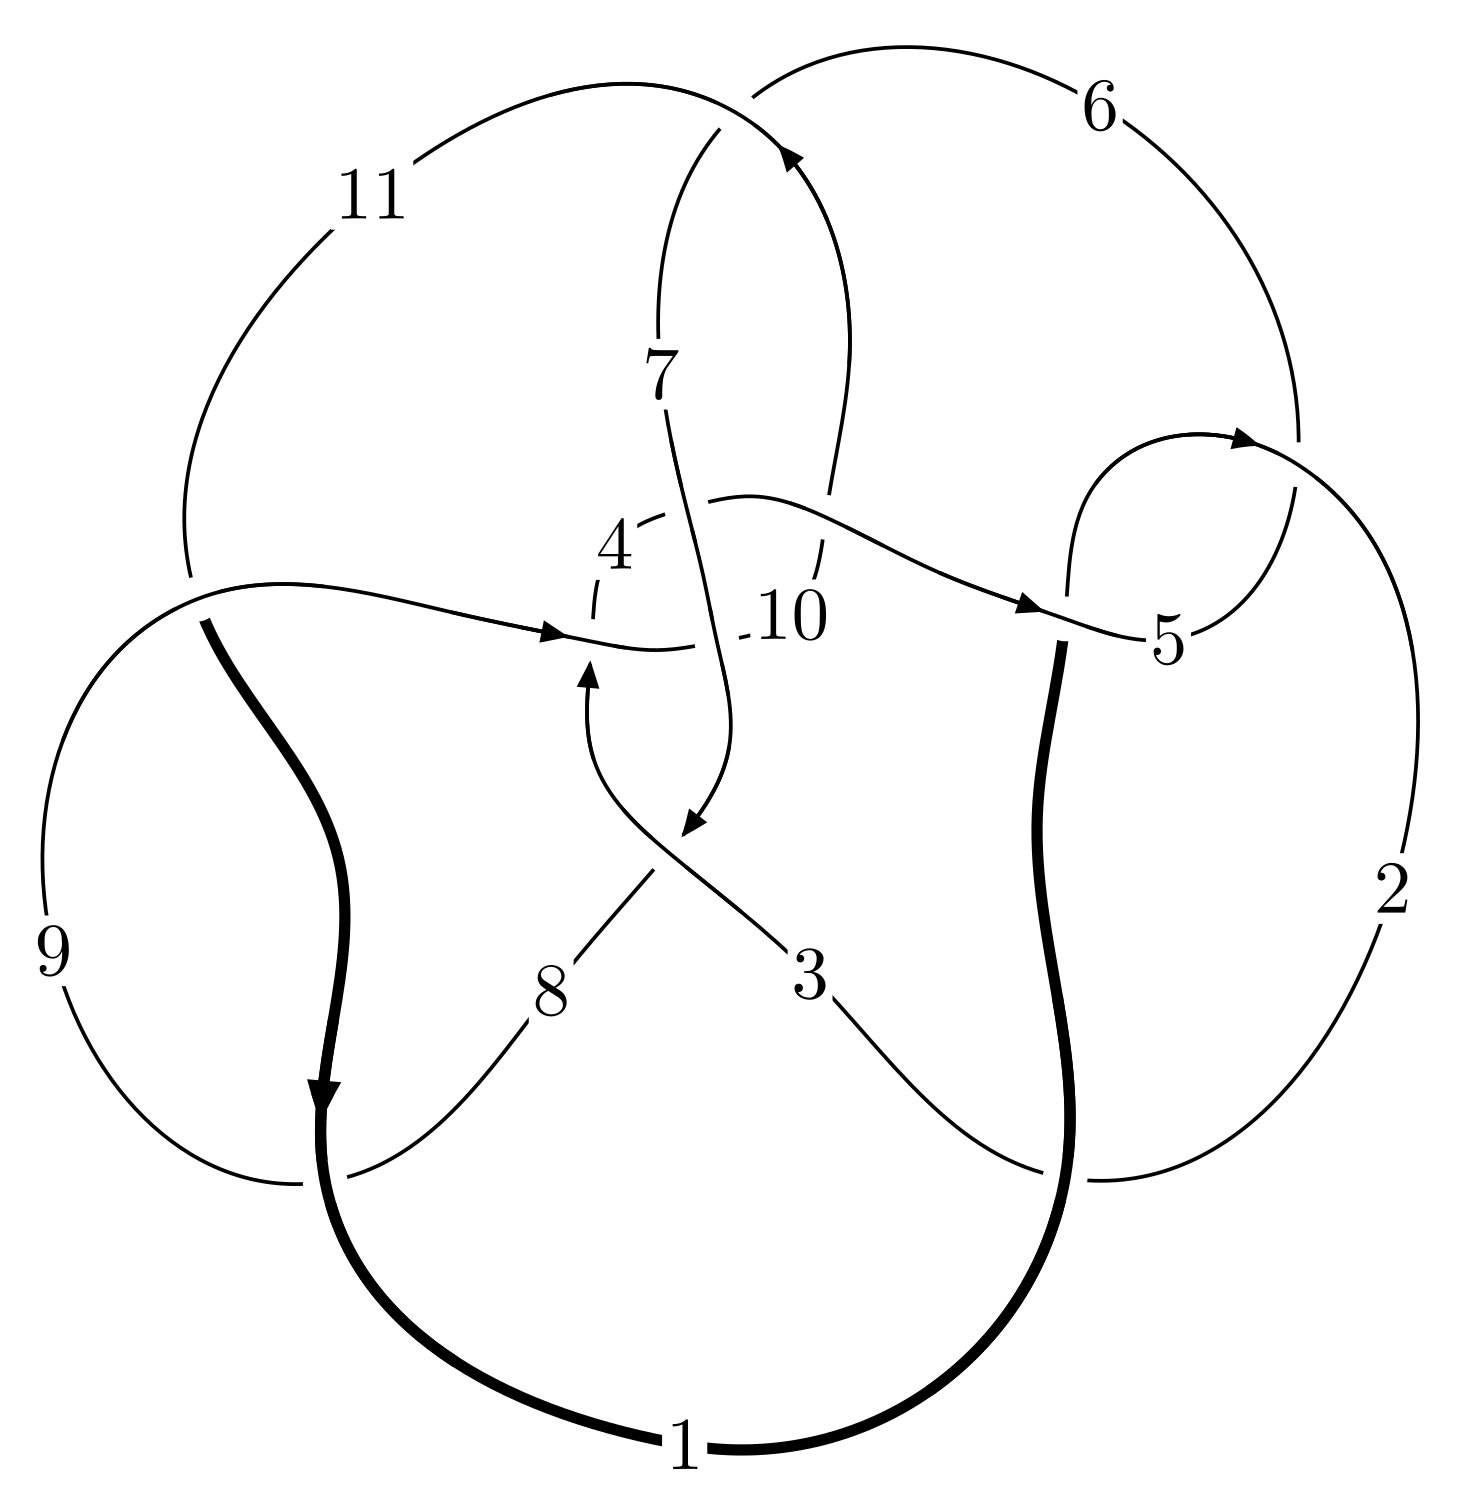
\includegraphics[width=112pt]{../../../GIT/diagram.site/Diagrams/png/711_11n_95.png}\\
\ \ \ A knot diagram\footnotemark}&
\allowdisplaybreaks
\textbf{Linearized knot diagam} \\
\cline{2-2}
 &
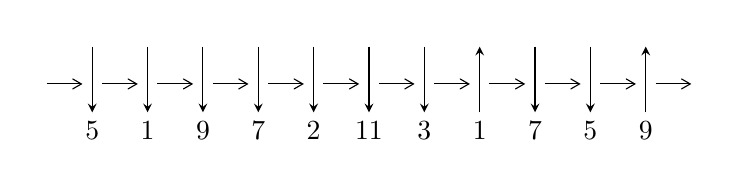
\begin{tikzpicture}[x=20pt, y=17pt]
	% nodes
	\node (C0) at (0, 0) {};
	\node (C1) at (1, 0) {};
	\node (C1U) at (1, +1) {};
	\node (C1D) at (1, -1) {5};

	\node (C2) at (2, 0) {};
	\node (C2U) at (2, +1) {};
	\node (C2D) at (2, -1) {1};

	\node (C3) at (3, 0) {};
	\node (C3U) at (3, +1) {};
	\node (C3D) at (3, -1) {9};

	\node (C4) at (4, 0) {};
	\node (C4U) at (4, +1) {};
	\node (C4D) at (4, -1) {7};

	\node (C5) at (5, 0) {};
	\node (C5U) at (5, +1) {};
	\node (C5D) at (5, -1) {2};

	\node (C6) at (6, 0) {};
	\node (C6U) at (6, +1) {};
	\node (C6D) at (6, -1) {11};

	\node (C7) at (7, 0) {};
	\node (C7U) at (7, +1) {};
	\node (C7D) at (7, -1) {3};

	\node (C8) at (8, 0) {};
	\node (C8U) at (8, +1) {};
	\node (C8D) at (8, -1) {1};

	\node (C9) at (9, 0) {};
	\node (C9U) at (9, +1) {};
	\node (C9D) at (9, -1) {7};

	\node (C10) at (10, 0) {};
	\node (C10U) at (10, +1) {};
	\node (C10D) at (10, -1) {5};

	\node (C11) at (11, 0) {};
	\node (C11U) at (11, +1) {};
	\node (C11D) at (11, -1) {9};
	\node (C12) at (12, 0) {};

	% arrows
	\draw[->,>={angle 60}]
	(C0) edge (C1) (C1) edge (C2) (C2) edge (C3) (C3) edge (C4) (C4) edge (C5) (C5) edge (C6) (C6) edge (C7) (C7) edge (C8) (C8) edge (C9) (C9) edge (C10) (C10) edge (C11) (C11) edge (C12) ;	\draw[->,>=stealth]
	(C1U) edge (C1D) (C2U) edge (C2D) (C3U) edge (C3D) (C4U) edge (C4D) (C5U) edge (C5D) (C6U) edge (C6D) (C7U) edge (C7D) (C8D) edge (C8U) (C9U) edge (C9D) (C10U) edge (C10D) (C11D) edge (C11U) ;
	\end{tikzpicture} \\
\hhline{~~} \\& 
\textbf{Solving Sequence} \\ \cline{2-2} 
 &
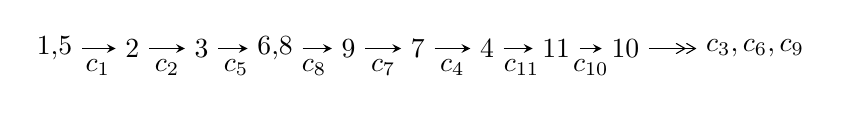
\begin{tikzpicture}[x=25pt, y=7pt]
	% node
	\node (A0) at (-1/8, 0) {1,5};
	\node (A1) at (1, 0) {2};
	\node (A2) at (2, 0) {3};
	\node (A3) at (49/16, 0) {6,8};
	\node (A4) at (33/8, 0) {9};
	\node (A5) at (41/8, 0) {7};
	\node (A6) at (49/8, 0) {4};
	\node (A7) at (57/8, 0) {11};
	\node (A8) at (65/8, 0) {10};
	\node (C1) at (1/2, -1) {$c_{1}$};
	\node (C2) at (3/2, -1) {$c_{2}$};
	\node (C3) at (5/2, -1) {$c_{5}$};
	\node (C4) at (29/8, -1) {$c_{8}$};
	\node (C5) at (37/8, -1) {$c_{7}$};
	\node (C6) at (45/8, -1) {$c_{4}$};
	\node (C7) at (53/8, -1) {$c_{11}$};
	\node (C8) at (61/8, -1) {$c_{10}$};
	\node (A9) at (10, 0) {$c_{3},c_{6},c_{9}$};

	% edge
	\draw[->,>=stealth]	
	(A0) edge (A1) (A1) edge (A2) (A2) edge (A3) (A3) edge (A4) (A4) edge (A5) (A5) edge (A6) (A6) edge (A7) (A7) edge (A8) ;
	\draw[->>,>={angle 60}]	
	(A8) edge (A9);
\end{tikzpicture} \\ 

\end{tabular} \\

\footnotetext{
The image of knot diagram is generated by the software ``\textbf{Draw programme}" developed by Andrew Bartholomew(\url{http://www.layer8.co.uk/maths/draw/index.htm\#Running-draw}), where we modified some parts for our purpose(\url{https://github.com/CATsTAILs/LinksPainter}).
}\phantom \\ \newline 
\centering \textbf{Ideals for irreducible components\footnotemark of $X_{\text{par}}$} 
 
\begin{align*}
I^u_{1}&=\langle 
u^{10}-4 u^9+5 u^8+4 u^7-20 u^6+24 u^5-8 u^4-8 u^3+7 u^2+b-1,\\
\phantom{I^u_{1}}&\phantom{= \langle  }u^{11}-7 u^{10}+18 u^9-12 u^8-36 u^7+95 u^6-84 u^5-2 u^4+59 u^3-31 u^2+2 a-9 u+9,\\
\phantom{I^u_{1}}&\phantom{= \langle  }u^{12}-5 u^{11}+10 u^{10}-4 u^9-22 u^8+51 u^7-48 u^6+10 u^5+23 u^4-21 u^3+3 u^2+5 u-2\rangle \\
I^u_{2}&=\langle 
u^5+2 u^4-2 u^2+b- u+1,\;-3 u^5-5 u^4+2 u^3+8 u^2+a+2 u-6,\;u^6+2 u^5-3 u^3-2 u^2+2 u+1\rangle \\
I^u_{3}&=\langle 
-4 u^4 a-5 u^3 a-10 u^4-4 u^2 a-7 u^3+3 a u+u^2+11 b+5 a+13 u-4,\\
\phantom{I^u_{3}}&\phantom{= \langle  }-6 u^4+u^2 a-2 u^3+a^2+2 a u+3 u^2+a+9 u-11,\;u^5+u^4- u^2+u+1\rangle \\
\\
\end{align*}
\raggedright * 3 irreducible components of $\dim_{\mathbb{C}}=0$, with total 28 representations.\\
\footnotetext{All coefficients of polynomials are rational numbers. But the coefficients are sometimes approximated in decimal forms when there is not enough margin.}
\newpage
\renewcommand{\arraystretch}{1}
\centering \section*{I. $I^u_{1}= \langle u^{10}-4 u^9+\cdots+b-1,\;u^{11}-7 u^{10}+\cdots+2 a+9,\;u^{12}-5 u^{11}+\cdots+5 u-2 \rangle$}
\flushleft \textbf{(i) Arc colorings}\\
\begin{tabular}{m{7pt} m{180pt} m{7pt} m{180pt} }
\flushright $a_{1}=$&$\begin{pmatrix}1\\0\end{pmatrix}$ \\
\flushright $a_{5}=$&$\begin{pmatrix}0\\u\end{pmatrix}$ \\
\flushright $a_{2}=$&$\begin{pmatrix}1\\u^2\end{pmatrix}$ \\
\flushright $a_{3}=$&$\begin{pmatrix}- u^2+1\\u^2\end{pmatrix}$ \\
\flushright $a_{6}=$&$\begin{pmatrix}- u\\- u^3+u\end{pmatrix}$ \\
\flushright $a_{8}=$&$\begin{pmatrix}-\frac{1}{2} u^{11}+\frac{7}{2} u^{10}+\cdots+\frac{9}{2} u-\frac{9}{2}\\- u^{10}+4 u^9-5 u^8-4 u^7+20 u^6-24 u^5+8 u^4+8 u^3-7 u^2+1\end{pmatrix}$ \\
\flushright $a_{9}=$&$\begin{pmatrix}-\frac{1}{2} u^{11}+\frac{5}{2} u^{10}+\cdots+\frac{9}{2} u-\frac{7}{2}\\- u^{10}+4 u^9-5 u^8-4 u^7+20 u^6-24 u^5+8 u^4+8 u^3-7 u^2+1\end{pmatrix}$ \\
\flushright $a_{7}=$&$\begin{pmatrix}-\frac{3}{2} u^{11}+\frac{13}{2} u^{10}+\cdots+\frac{11}{2} u-\frac{7}{2}\\u^{11}-4 u^{10}+6 u^9+u^8-18 u^7+30 u^6-22 u^5+2 u^4+9 u^3-6 u^2+1\end{pmatrix}$ \\
\flushright $a_{4}=$&$\begin{pmatrix}-\frac{1}{2} u^{11}+\frac{3}{2} u^{10}+\cdots+\frac{1}{2} u+\frac{1}{2}\\u^{10}-3 u^9+2 u^8+6 u^7-14 u^6+11 u^5+2 u^4-8 u^3+4 u^2+2 u-1\end{pmatrix}$ \\
\flushright $a_{11}=$&$\begin{pmatrix}\frac{3}{2} u^{11}-\frac{13}{2} u^{10}+\cdots-\frac{11}{2} u+\frac{7}{2}\\- u^{11}+4 u^{10}+\cdots+3 u-1\end{pmatrix}$ \\
\flushright $a_{10}=$&$\begin{pmatrix}\frac{3}{2} u^{11}-\frac{13}{2} u^{10}+\cdots-\frac{11}{2} u+\frac{7}{2}\\- u^{11}+5 u^{10}+\cdots+5 u-3\end{pmatrix}$\\ \flushright $a_{10}=$&$\begin{pmatrix}\frac{3}{2} u^{11}-\frac{13}{2} u^{10}+\cdots-\frac{11}{2} u+\frac{7}{2}\\- u^{11}+5 u^{10}+\cdots+5 u-3\end{pmatrix}$\\&\end{tabular}
\flushleft \textbf{(ii) Obstruction class $= -1$}\\~\\
\flushleft \textbf{(iii) Cusp Shapes $= - u^{11}+6 u^{10}-14 u^9+9 u^8+27 u^7-75 u^6+75 u^5-10 u^4-49 u^3+40 u^2-18$}\\~\\
\newpage\renewcommand{\arraystretch}{1}
\flushleft \textbf{(iv) u-Polynomials at the component}\newline \\
\begin{tabular}{m{50pt}|m{274pt}}
Crossings & \hspace{64pt}u-Polynomials at each crossing \\
\hline $$\begin{aligned}c_{1},c_{5}\end{aligned}$$&$\begin{aligned}
&u^{12}+5 u^{11}+\cdots-5 u-2
\end{aligned}$\\
\hline $$\begin{aligned}c_{2}\end{aligned}$$&$\begin{aligned}
&u^{12}+5 u^{11}+\cdots+37 u+4
\end{aligned}$\\
\hline $$\begin{aligned}c_{3},c_{4},c_{10}\end{aligned}$$&$\begin{aligned}
&u^{12}- u^{11}+\cdots-2 u-1
\end{aligned}$\\
\hline $$\begin{aligned}c_{6}\end{aligned}$$&$\begin{aligned}
&u^{12}+12 u^{11}+\cdots+240 u+32
\end{aligned}$\\
\hline $$\begin{aligned}c_{7}\end{aligned}$$&$\begin{aligned}
&u^{12}+5 u^{10}+\cdots+4 u+1
\end{aligned}$\\
\hline $$\begin{aligned}c_{8},c_{11}\end{aligned}$$&$\begin{aligned}
&u^{12}+2 u^{11}+\cdots+3 u+1
\end{aligned}$\\
\hline $$\begin{aligned}c_{9}\end{aligned}$$&$\begin{aligned}
&u^{12}-7 u^{11}+\cdots-15 u-4
\end{aligned}$\\
\hline
\end{tabular}\\~\\
\newpage\renewcommand{\arraystretch}{1}
\flushleft \textbf{(v) Riley Polynomials at the component}\newline \\
\begin{tabular}{m{50pt}|m{274pt}}
Crossings & \hspace{64pt}Riley Polynomials at each crossing \\
\hline $$\begin{aligned}c_{1},c_{5}\end{aligned}$$&$\begin{aligned}
&y^{12}-5 y^{11}+\cdots-37 y+4
\end{aligned}$\\
\hline $$\begin{aligned}c_{2}\end{aligned}$$&$\begin{aligned}
&y^{12}+7 y^{11}+\cdots-353 y+16
\end{aligned}$\\
\hline $$\begin{aligned}c_{3},c_{4},c_{10}\end{aligned}$$&$\begin{aligned}
&y^{12}-19 y^{11}+\cdots+2 y+1
\end{aligned}$\\
\hline $$\begin{aligned}c_{6}\end{aligned}$$&$\begin{aligned}
&y^{12}-6 y^{11}+\cdots-7936 y+1024
\end{aligned}$\\
\hline $$\begin{aligned}c_{7}\end{aligned}$$&$\begin{aligned}
&y^{12}+10 y^{11}+\cdots-10 y+1
\end{aligned}$\\
\hline $$\begin{aligned}c_{8},c_{11}\end{aligned}$$&$\begin{aligned}
&y^{12}-6 y^{11}+\cdots-25 y+1
\end{aligned}$\\
\hline $$\begin{aligned}c_{9}\end{aligned}$$&$\begin{aligned}
&y^{12}-3 y^{11}+\cdots-689 y+16
\end{aligned}$\\
\hline
\end{tabular}\\~\\
\newpage\flushleft \textbf{(vi) Complex Volumes and Cusp Shapes}
$$\begin{array}{c|c|c}  
\text{Solutions to }I^u_{1}& \I (\text{vol} + \sqrt{-1}CS) & \text{Cusp shape}\\
 \hline 
\begin{aligned}
u &= \phantom{-}0.634055 + 0.761588 I \\
a &= \phantom{-}2.40907 - 0.56101 I \\
b &= -1.061820 + 0.403224 I\end{aligned}
 & \phantom{-}2.28232 - 3.09531 I & -6.37045 + 4.07458 I \\ \hline\begin{aligned}
u &= \phantom{-}0.634055 - 0.761588 I \\
a &= \phantom{-}2.40907 + 0.56101 I \\
b &= -1.061820 - 0.403224 I\end{aligned}
 & \phantom{-}2.28232 + 3.09531 I & -6.37045 - 4.07458 I \\ \hline\begin{aligned}
u &= \phantom{-}0.706953 + 1.119620 I \\
a &= -2.03790 - 1.24403 I \\
b &= \phantom{-}1.33004 + 0.60517 I\end{aligned}
 & -1.55271 + 4.05634 I & -6.99284 - 2.54487 I \\ \hline\begin{aligned}
u &= \phantom{-}0.706953 - 1.119620 I \\
a &= -2.03790 + 1.24403 I \\
b &= \phantom{-}1.33004 - 0.60517 I\end{aligned}
 & -1.55271 - 4.05634 I & -6.99284 + 2.54487 I \\ \hline\begin{aligned}
u &= \phantom{-}1.184170 + 0.621257 I \\
a &= \phantom{-}1.075910 + 0.634900 I \\
b &= -0.732377 + 0.158790 I\end{aligned}
 & \phantom{-}0.53240 - 2.26677 I & -5.92780 + 2.45213 I \\ \hline\begin{aligned}
u &= \phantom{-}1.184170 - 0.621257 I \\
a &= \phantom{-}1.075910 - 0.634900 I \\
b &= -0.732377 - 0.158790 I\end{aligned}
 & \phantom{-}0.53240 + 2.26677 I & -5.92780 - 2.45213 I \\ \hline\begin{aligned}
u &= -0.585422 + 0.102144 I \\
a &= \phantom{-}0.251345 - 0.127948 I \\
b &= -0.388763 - 1.056570 I\end{aligned}
 & -0.76434 + 2.25567 I & -2.25761 - 1.65555 I \\ \hline\begin{aligned}
u &= -0.585422 - 0.102144 I \\
a &= \phantom{-}0.251345 + 0.127948 I \\
b &= -0.388763 + 1.056570 I\end{aligned}
 & -0.76434 - 2.25567 I & -2.25761 + 1.65555 I \\ \hline\begin{aligned}
u &= \phantom{-}1.13630 + 0.87513 I \\
a &= -2.57645 + 0.49107 I \\
b &= \phantom{-}1.35172 - 1.03292 I\end{aligned}
 & -2.90723 - 11.19710 I & -8.74463 + 6.08532 I \\ \hline\begin{aligned}
u &= \phantom{-}1.13630 - 0.87513 I \\
a &= -2.57645 - 0.49107 I \\
b &= \phantom{-}1.35172 + 1.03292 I\end{aligned}
 & -2.90723 + 11.19710 I & -8.74463 - 6.08532 I\\
 \hline 
 \end{array}$$\newpage$$\begin{array}{c|c|c}  
\text{Solutions to }I^u_{1}& \I (\text{vol} + \sqrt{-1}CS) & \text{Cusp shape}\\
 \hline 
\begin{aligned}
u &= \phantom{-}0.531194\phantom{ +0.000000I} \\
a &= -1.14054\phantom{ +0.000000I} \\
b &= \phantom{-}0.227398\phantom{ +0.000000I}\end{aligned}
 & -0.766539\phantom{ +0.000000I} & -13.0250\phantom{ +0.000000I} \\ \hline\begin{aligned}
u &= -1.68330\phantom{ +0.000000I} \\
a &= -0.603416\phantom{ +0.000000I} \\
b &= \phantom{-}0.774996\phantom{ +0.000000I}\end{aligned}
 & -10.8637\phantom{ +0.000000I} & -2.38840\phantom{ +0.000000I}\\
 \hline 
 \end{array}$$\newpage\newpage\renewcommand{\arraystretch}{1}
\centering \section*{II. $I^u_{2}= \langle u^5+2 u^4-2 u^2+b- u+1,\;-3 u^5-5 u^4+2 u^3+8 u^2+a+2 u-6,\;u^6+2 u^5-3 u^3-2 u^2+2 u+1 \rangle$}
\flushleft \textbf{(i) Arc colorings}\\
\begin{tabular}{m{7pt} m{180pt} m{7pt} m{180pt} }
\flushright $a_{1}=$&$\begin{pmatrix}1\\0\end{pmatrix}$ \\
\flushright $a_{5}=$&$\begin{pmatrix}0\\u\end{pmatrix}$ \\
\flushright $a_{2}=$&$\begin{pmatrix}1\\u^2\end{pmatrix}$ \\
\flushright $a_{3}=$&$\begin{pmatrix}- u^2+1\\u^2\end{pmatrix}$ \\
\flushright $a_{6}=$&$\begin{pmatrix}- u\\- u^3+u\end{pmatrix}$ \\
\flushright $a_{8}=$&$\begin{pmatrix}3 u^5+5 u^4-2 u^3-8 u^2-2 u+6\\- u^5-2 u^4+2 u^2+u-1\end{pmatrix}$ \\
\flushright $a_{9}=$&$\begin{pmatrix}2 u^5+3 u^4-2 u^3-6 u^2- u+5\\- u^5-2 u^4+2 u^2+u-1\end{pmatrix}$ \\
\flushright $a_{7}=$&$\begin{pmatrix}2 u^5+3 u^4- u^3-5 u^2-2 u+4\\- u^5-2 u^4- u^3+2 u^2+2 u-1\end{pmatrix}$ \\
\flushright $a_{4}=$&$\begin{pmatrix}-3 u^5-5 u^4+2 u^3+8 u^2+3 u-7\\u^5+2 u^4-2 u^2- u+2\end{pmatrix}$ \\
\flushright $a_{11}=$&$\begin{pmatrix}-2 u^5-3 u^4+u^3+5 u^2+2 u-4\\- u^2- u+1\end{pmatrix}$ \\
\flushright $a_{10}=$&$\begin{pmatrix}-2 u^5-3 u^4+u^3+5 u^2+2 u-4\\u^5+u^4- u^3-3 u^2- u+2\end{pmatrix}$\\ \flushright $a_{10}=$&$\begin{pmatrix}-2 u^5-3 u^4+u^3+5 u^2+2 u-4\\u^5+u^4- u^3-3 u^2- u+2\end{pmatrix}$\\&\end{tabular}
\flushleft \textbf{(ii) Obstruction class $= 1$}\\~\\
\flushleft \textbf{(iii) Cusp Shapes $= 4 u^5+7 u^4+4 u^3-6 u^2-9 u-7$}\\~\\
\newpage\renewcommand{\arraystretch}{1}
\flushleft \textbf{(iv) u-Polynomials at the component}\newline \\
\begin{tabular}{m{50pt}|m{274pt}}
Crossings & \hspace{64pt}u-Polynomials at each crossing \\
\hline $$\begin{aligned}c_{1}\end{aligned}$$&$\begin{aligned}
&u^6+2 u^5-3 u^3-2 u^2+2 u+1
\end{aligned}$\\
\hline $$\begin{aligned}c_{2}\end{aligned}$$&$\begin{aligned}
&u^6+4 u^5+8 u^4+15 u^3+16 u^2+8 u+1
\end{aligned}$\\
\hline $$\begin{aligned}c_{3}\end{aligned}$$&$\begin{aligned}
&u^6+u^5-2 u^4-3 u^3-5 u^2-4 u-1
\end{aligned}$\\
\hline $$\begin{aligned}c_{4},c_{10}\end{aligned}$$&$\begin{aligned}
&u^6- u^5-2 u^4+3 u^3-5 u^2+4 u-1
\end{aligned}$\\
\hline $$\begin{aligned}c_{5}\end{aligned}$$&$\begin{aligned}
&u^6-2 u^5+3 u^3-2 u^2-2 u+1
\end{aligned}$\\
\hline $$\begin{aligned}c_{6}\end{aligned}$$&$\begin{aligned}
&u^6+u^5-2 u^4+2 u^3-2 u+1
\end{aligned}$\\
\hline $$\begin{aligned}c_{7}\end{aligned}$$&$\begin{aligned}
&u^6-4 u^3-5 u^2-2 u-1
\end{aligned}$\\
\hline $$\begin{aligned}c_{8}\end{aligned}$$&$\begin{aligned}
&u^6+2 u^5-2 u^3-2 u^2- u+1
\end{aligned}$\\
\hline $$\begin{aligned}c_{9}\end{aligned}$$&$\begin{aligned}
&u^6+4 u^5+5 u^4+2 u^3- u^2- u+1
\end{aligned}$\\
\hline $$\begin{aligned}c_{11}\end{aligned}$$&$\begin{aligned}
&u^6-2 u^5+2 u^3-2 u^2+u+1
\end{aligned}$\\
\hline
\end{tabular}\\~\\
\newpage\renewcommand{\arraystretch}{1}
\flushleft \textbf{(v) Riley Polynomials at the component}\newline \\
\begin{tabular}{m{50pt}|m{274pt}}
Crossings & \hspace{64pt}Riley Polynomials at each crossing \\
\hline $$\begin{aligned}c_{1},c_{5}\end{aligned}$$&$\begin{aligned}
&y^6-4 y^5+8 y^4-15 y^3+16 y^2-8 y+1
\end{aligned}$\\
\hline $$\begin{aligned}c_{2}\end{aligned}$$&$\begin{aligned}
&y^6-24 y^4-31 y^3+32 y^2-32 y+1
\end{aligned}$\\
\hline $$\begin{aligned}c_{3},c_{4},c_{10}\end{aligned}$$&$\begin{aligned}
&y^6-5 y^5+17 y^3+5 y^2-6 y+1
\end{aligned}$\\
\hline $$\begin{aligned}c_{6}\end{aligned}$$&$\begin{aligned}
&y^6-5 y^5+2 y^3+4 y^2-4 y+1
\end{aligned}$\\
\hline $$\begin{aligned}c_{7}\end{aligned}$$&$\begin{aligned}
&y^6-10 y^4-18 y^3+9 y^2+6 y+1
\end{aligned}$\\
\hline $$\begin{aligned}c_{8},c_{11}\end{aligned}$$&$\begin{aligned}
&y^6-4 y^5+4 y^4+2 y^3-5 y+1
\end{aligned}$\\
\hline $$\begin{aligned}c_{9}\end{aligned}$$&$\begin{aligned}
&y^6-6 y^5+7 y^4-4 y^3+15 y^2-3 y+1
\end{aligned}$\\
\hline
\end{tabular}\\~\\
\newpage\flushleft \textbf{(vi) Complex Volumes and Cusp Shapes}
$$\begin{array}{c|c|c}  
\text{Solutions to }I^u_{2}& \I (\text{vol} + \sqrt{-1}CS) & \text{Cusp shape}\\
 \hline 
\begin{aligned}
u &= \phantom{-}0.907957 + 0.227043 I \\
a &= -0.348496 + 0.361180 I \\
b &= \phantom{-}0.355765 - 0.898533 I\end{aligned}
 & -1.45069 - 2.49752 I & -13.4121 + 4.8455 I \\ \hline\begin{aligned}
u &= \phantom{-}0.907957 - 0.227043 I \\
a &= -0.348496 - 0.361180 I \\
b &= \phantom{-}0.355765 + 0.898533 I\end{aligned}
 & -1.45069 + 2.49752 I & -13.4121 - 4.8455 I \\ \hline\begin{aligned}
u &= -0.934823 + 0.946305 I \\
a &= -2.43499 + 0.27700 I \\
b &= \phantom{-}1.42809 + 0.28813 I\end{aligned}
 & \phantom{-}5.64849 + 3.45368 I & -2.17386 - 2.96497 I \\ \hline\begin{aligned}
u &= -0.934823 - 0.946305 I \\
a &= -2.43499 - 0.27700 I \\
b &= \phantom{-}1.42809 - 0.28813 I\end{aligned}
 & \phantom{-}5.64849 - 3.45368 I & -2.17386 + 2.96497 I \\ \hline\begin{aligned}
u &= -1.52247\phantom{ +0.000000I} \\
a &= -0.116304\phantom{ +0.000000I} \\
b &= -0.452275\phantom{ +0.000000I}\end{aligned}
 & -11.4632\phantom{ +0.000000I} & -16.4310\phantom{ +0.000000I} \\ \hline\begin{aligned}
u &= -0.423796\phantom{ +0.000000I} \\
a &= \phantom{-}5.68327\phantom{ +0.000000I} \\
b &= -1.11543\phantom{ +0.000000I}\end{aligned}
 & -6.80200\phantom{ +0.000000I} & -4.39680\phantom{ +0.000000I}\\
 \hline 
 \end{array}$$\newpage\newpage\renewcommand{\arraystretch}{1}
\centering \section*{III. $I^u_{3}= \langle -4 u^4 a-10 u^4+\cdots+5 a-4,\;-6 u^4-2 u^3+\cdots+a-11,\;u^5+u^4- u^2+u+1 \rangle$}
\flushleft \textbf{(i) Arc colorings}\\
\begin{tabular}{m{7pt} m{180pt} m{7pt} m{180pt} }
\flushright $a_{1}=$&$\begin{pmatrix}1\\0\end{pmatrix}$ \\
\flushright $a_{5}=$&$\begin{pmatrix}0\\u\end{pmatrix}$ \\
\flushright $a_{2}=$&$\begin{pmatrix}1\\u^2\end{pmatrix}$ \\
\flushright $a_{3}=$&$\begin{pmatrix}- u^2+1\\u^2\end{pmatrix}$ \\
\flushright $a_{6}=$&$\begin{pmatrix}- u\\- u^3+u\end{pmatrix}$ \\
\flushright $a_{8}=$&$\begin{pmatrix}a\\0.363636 a u^{4}+0.909091 u^{4}+\cdots-0.454545 a+0.363636\end{pmatrix}$ \\
\flushright $a_{9}=$&$\begin{pmatrix}0.363636 a u^{4}+0.909091 u^{4}+\cdots+0.545455 a+0.363636\\0.363636 a u^{4}+0.909091 u^{4}+\cdots-0.454545 a+0.363636\end{pmatrix}$ \\
\flushright $a_{7}=$&$\begin{pmatrix}0.272727 a u^{4}+0.181818 u^{4}+\cdots+0.909091 a+0.272727\\0.181818 a u^{4}+1.45455 u^{4}+\cdots-0.727273 a+0.181818\end{pmatrix}$ \\
\flushright $a_{4}=$&$\begin{pmatrix}-0.454545 a u^{4}-3.63636 u^{4}+\cdots-0.181818 a-2.45455\\0.0909091 a u^{4}+1.72727 u^{4}+\cdots-0.363636 a+1.09091\end{pmatrix}$ \\
\flushright $a_{11}=$&$\begin{pmatrix}0.272727 a u^{4}+0.181818 u^{4}+\cdots+0.909091 a+0.272727\\0.181818 a u^{4}+1.45455 u^{4}+\cdots-0.727273 a+0.181818\end{pmatrix}$ \\
\flushright $a_{10}=$&$\begin{pmatrix}0.272727 a u^{4}+0.181818 u^{4}+\cdots+0.909091 a+0.272727\\-0.272727 a u^{4}+0.818182 u^{4}+\cdots-0.909091 a+0.727273\end{pmatrix}$\\ \flushright $a_{10}=$&$\begin{pmatrix}0.272727 a u^{4}+0.181818 u^{4}+\cdots+0.909091 a+0.272727\\-0.272727 a u^{4}+0.818182 u^{4}+\cdots-0.909091 a+0.727273\end{pmatrix}$\\&\end{tabular}
\flushleft \textbf{(ii) Obstruction class $= -1$}\\~\\
\flushleft \textbf{(iii) Cusp Shapes $= -4 u^4+4 u^2+4 u-18$}\\~\\
\newpage\renewcommand{\arraystretch}{1}
\flushleft \textbf{(iv) u-Polynomials at the component}\newline \\
\begin{tabular}{m{50pt}|m{274pt}}
Crossings & \hspace{64pt}u-Polynomials at each crossing \\
\hline $$\begin{aligned}c_{1},c_{5}\end{aligned}$$&$\begin{aligned}
&(u^5- u^4+u^2+u-1)^2
\end{aligned}$\\
\hline $$\begin{aligned}c_{2}\end{aligned}$$&$\begin{aligned}
&(u^5+u^4+4 u^3+3 u^2+3 u+1)^2
\end{aligned}$\\
\hline $$\begin{aligned}c_{3},c_{4},c_{10}\end{aligned}$$&$\begin{aligned}
&u^{10}+u^9-4 u^8-4 u^7-2 u^6+2 u^5+29 u^4+7 u^3-48 u^2+12 u-1
\end{aligned}$\\
\hline $$\begin{aligned}c_{6}\end{aligned}$$&$\begin{aligned}
&(u-1)^{10}
\end{aligned}$\\
\hline $$\begin{aligned}c_{7}\end{aligned}$$&$\begin{aligned}
&u^{10}+u^9+2 u^8+6 u^7-14 u^6+28 u^5-59 u^4+53 u^3-82 u^2+34 u-13
\end{aligned}$\\
\hline $$\begin{aligned}c_{8},c_{11}\end{aligned}$$&$\begin{aligned}
&u^{10}+3 u^9+2 u^8-8 u^7-24 u^6-16 u^5+25 u^4+71 u^3+78 u^2+40 u+7
\end{aligned}$\\
\hline $$\begin{aligned}c_{9}\end{aligned}$$&$\begin{aligned}
&(u^5+3 u^4-5 u^2- u+3)^2
\end{aligned}$\\
\hline
\end{tabular}\\~\\
\newpage\renewcommand{\arraystretch}{1}
\flushleft \textbf{(v) Riley Polynomials at the component}\newline \\
\begin{tabular}{m{50pt}|m{274pt}}
Crossings & \hspace{64pt}Riley Polynomials at each crossing \\
\hline $$\begin{aligned}c_{1},c_{5}\end{aligned}$$&$\begin{aligned}
&(y^5- y^4+4 y^3-3 y^2+3 y-1)^2
\end{aligned}$\\
\hline $$\begin{aligned}c_{2}\end{aligned}$$&$\begin{aligned}
&(y^5+7 y^4+16 y^3+13 y^2+3 y-1)^2
\end{aligned}$\\
\hline $$\begin{aligned}c_{3},c_{4},c_{10}\end{aligned}$$&$\begin{aligned}
&y^{10}-9 y^9+\cdots-48 y+1
\end{aligned}$\\
\hline $$\begin{aligned}c_{6}\end{aligned}$$&$\begin{aligned}
&(y-1)^{10}
\end{aligned}$\\
\hline $$\begin{aligned}c_{7}\end{aligned}$$&$\begin{aligned}
&y^{10}+3 y^9+\cdots+976 y+169
\end{aligned}$\\
\hline $$\begin{aligned}c_{8},c_{11}\end{aligned}$$&$\begin{aligned}
&y^{10}-5 y^9+\cdots-508 y+49
\end{aligned}$\\
\hline $$\begin{aligned}c_{9}\end{aligned}$$&$\begin{aligned}
&(y^5-9 y^4+28 y^3-43 y^2+31 y-9)^2
\end{aligned}$\\
\hline
\end{tabular}\\~\\
\newpage\flushleft \textbf{(vi) Complex Volumes and Cusp Shapes}
$$\begin{array}{c|c|c}  
\text{Solutions to }I^u_{3}& \I (\text{vol} + \sqrt{-1}CS) & \text{Cusp shape}\\
 \hline 
\begin{aligned}
u &= \phantom{-}0.758138 + 0.584034 I \\
a &= -1.87197 - 0.03044 I \\
b &= \phantom{-}0.452332 - 1.123840 I\end{aligned}
 & -4.75993 - 2.21397 I & -11.11432 + 4.22289 I \\ \hline\begin{aligned}
u &= \phantom{-}0.758138 + 0.584034 I \\
a &= -0.87798 - 2.02319 I \\
b &= \phantom{-}0.81806 + 1.53771 I\end{aligned}
 & -4.75993 - 2.21397 I & -11.11432 + 4.22289 I \\ \hline\begin{aligned}
u &= \phantom{-}0.758138 - 0.584034 I \\
a &= -1.87197 + 0.03044 I \\
b &= \phantom{-}0.452332 + 1.123840 I\end{aligned}
 & -4.75993 + 2.21397 I & -11.11432 - 4.22289 I \\ \hline\begin{aligned}
u &= \phantom{-}0.758138 - 0.584034 I \\
a &= -0.87798 + 2.02319 I \\
b &= \phantom{-}0.81806 - 1.53771 I\end{aligned}
 & -4.75993 + 2.21397 I & -11.11432 - 4.22289 I \\ \hline\begin{aligned}
u &= -0.935538 + 0.903908 I \\
a &= -1.88766 + 0.16400 I \\
b &= \phantom{-}0.868620 + 0.215856 I\end{aligned}
 & \phantom{-}4.37856 + 3.33174 I & -10.08126 - 2.36228 I \\ \hline\begin{aligned}
u &= -0.935538 + 0.903908 I \\
a &= \phantom{-}2.70055 - 0.28054 I \\
b &= -1.72566 - 0.41266 I\end{aligned}
 & \phantom{-}4.37856 + 3.33174 I & -10.08126 - 2.36228 I \\ \hline\begin{aligned}
u &= -0.935538 - 0.903908 I \\
a &= -1.88766 - 0.16400 I \\
b &= \phantom{-}0.868620 - 0.215856 I\end{aligned}
 & \phantom{-}4.37856 - 3.33174 I & -10.08126 + 2.36228 I \\ \hline\begin{aligned}
u &= -0.935538 - 0.903908 I \\
a &= \phantom{-}2.70055 + 0.28054 I \\
b &= -1.72566 + 0.41266 I\end{aligned}
 & \phantom{-}4.37856 - 3.33174 I & -10.08126 + 2.36228 I \\ \hline\begin{aligned}
u &= -0.645200\phantom{ +0.000000I} \\
a &= \phantom{-}3.94511\phantom{ +0.000000I} \\
b &= \phantom{-}0.340045\phantom{ +0.000000I}\end{aligned}
 & -7.46192\phantom{ +0.000000I} & -19.6090\phantom{ +0.000000I} \\ \hline\begin{aligned}
u &= -0.645200\phantom{ +0.000000I} \\
a &= -4.07100\phantom{ +0.000000I} \\
b &= \phantom{-}1.83325\phantom{ +0.000000I}\end{aligned}
 & -7.46192\phantom{ +0.000000I} & -19.6090\phantom{ +0.000000I}\\
 \hline 
 \end{array}$$\newpage
\newpage\renewcommand{\arraystretch}{1}
\centering \section*{ IV. u-Polynomials}
\begin{tabular}{m{50pt}|m{274pt}}
Crossings & \hspace{64pt}u-Polynomials at each crossing \\
\hline $$\begin{aligned}c_{1}\end{aligned}$$&$\begin{aligned}
&(u^5- u^4+u^2+u-1)^2(u^6+2 u^5-3 u^3-2 u^2+2 u+1)\\
&\cdot(u^{12}+5 u^{11}+\cdots-5 u-2)
\end{aligned}$\\
\hline $$\begin{aligned}c_{2}\end{aligned}$$&$\begin{aligned}
&(u^5+u^4+4 u^3+3 u^2+3 u+1)^2\\
&\cdot(u^6+4 u^5+\cdots+8 u+1)(u^{12}+5 u^{11}+\cdots+37 u+4)
\end{aligned}$\\
\hline $$\begin{aligned}c_{3}\end{aligned}$$&$\begin{aligned}
&(u^6+u^5-2 u^4-3 u^3-5 u^2-4 u-1)\\
&\cdot(u^{10}+u^9-4 u^8-4 u^7-2 u^6+2 u^5+29 u^4+7 u^3-48 u^2+12 u-1)\\
&\cdot(u^{12}- u^{11}+\cdots-2 u-1)
\end{aligned}$\\
\hline $$\begin{aligned}c_{4},c_{10}\end{aligned}$$&$\begin{aligned}
&(u^6- u^5-2 u^4+3 u^3-5 u^2+4 u-1)\\
&\cdot(u^{10}+u^9-4 u^8-4 u^7-2 u^6+2 u^5+29 u^4+7 u^3-48 u^2+12 u-1)\\
&\cdot(u^{12}- u^{11}+\cdots-2 u-1)
\end{aligned}$\\
\hline $$\begin{aligned}c_{5}\end{aligned}$$&$\begin{aligned}
&(u^5- u^4+u^2+u-1)^2(u^6-2 u^5+3 u^3-2 u^2-2 u+1)\\
&\cdot(u^{12}+5 u^{11}+\cdots-5 u-2)
\end{aligned}$\\
\hline $$\begin{aligned}c_{6}\end{aligned}$$&$\begin{aligned}
&((u-1)^{10})(u^6+u^5+\cdots-2 u+1)(u^{12}+12 u^{11}+\cdots+240 u+32)
\end{aligned}$\\
\hline $$\begin{aligned}c_{7}\end{aligned}$$&$\begin{aligned}
&(u^6-4 u^3-5 u^2-2 u-1)\\
&\cdot(u^{10}+u^9+2 u^8+6 u^7-14 u^6+28 u^5-59 u^4+53 u^3-82 u^2+34 u-13)\\
&\cdot(u^{12}+5 u^{10}+\cdots+4 u+1)
\end{aligned}$\\
\hline $$\begin{aligned}c_{8}\end{aligned}$$&$\begin{aligned}
&(u^6+2 u^5-2 u^3-2 u^2- u+1)\\
&\cdot(u^{10}+3 u^9+2 u^8-8 u^7-24 u^6-16 u^5+25 u^4+71 u^3+78 u^2+40 u+7)\\
&\cdot(u^{12}+2 u^{11}+\cdots+3 u+1)
\end{aligned}$\\
\hline $$\begin{aligned}c_{9}\end{aligned}$$&$\begin{aligned}
&(u^5+3 u^4-5 u^2- u+3)^2(u^6+4 u^5+5 u^4+2 u^3- u^2- u+1)\\
&\cdot(u^{12}-7 u^{11}+\cdots-15 u-4)
\end{aligned}$\\
\hline $$\begin{aligned}c_{11}\end{aligned}$$&$\begin{aligned}
&(u^6-2 u^5+2 u^3-2 u^2+u+1)\\
&\cdot(u^{10}+3 u^9+2 u^8-8 u^7-24 u^6-16 u^5+25 u^4+71 u^3+78 u^2+40 u+7)\\
&\cdot(u^{12}+2 u^{11}+\cdots+3 u+1)
\end{aligned}$\\
\hline
\end{tabular}\newpage\renewcommand{\arraystretch}{1}
\centering \section*{ V. Riley Polynomials}
\begin{tabular}{m{50pt}|m{274pt}}
Crossings & \hspace{64pt}Riley Polynomials at each crossing \\
\hline $$\begin{aligned}c_{1},c_{5}\end{aligned}$$&$\begin{aligned}
&(y^5- y^4+4 y^3-3 y^2+3 y-1)^2\\
&\cdot(y^6-4 y^5+\cdots-8 y+1)(y^{12}-5 y^{11}+\cdots-37 y+4)
\end{aligned}$\\
\hline $$\begin{aligned}c_{2}\end{aligned}$$&$\begin{aligned}
&(y^5+7 y^4+16 y^3+13 y^2+3 y-1)^2\\
&\cdot(y^6-24 y^4+\cdots-32 y+1)(y^{12}+7 y^{11}+\cdots-353 y+16)
\end{aligned}$\\
\hline $$\begin{aligned}c_{3},c_{4},c_{10}\end{aligned}$$&$\begin{aligned}
&(y^6-5 y^5+17 y^3+5 y^2-6 y+1)(y^{10}-9 y^9+\cdots-48 y+1)\\
&\cdot(y^{12}-19 y^{11}+\cdots+2 y+1)
\end{aligned}$\\
\hline $$\begin{aligned}c_{6}\end{aligned}$$&$\begin{aligned}
&(y-1)^{10}(y^6-5 y^5+2 y^3+4 y^2-4 y+1)\\
&\cdot(y^{12}-6 y^{11}+\cdots-7936 y+1024)
\end{aligned}$\\
\hline $$\begin{aligned}c_{7}\end{aligned}$$&$\begin{aligned}
&(y^6-10 y^4-18 y^3+9 y^2+6 y+1)(y^{10}+3 y^9+\cdots+976 y+169)\\
&\cdot(y^{12}+10 y^{11}+\cdots-10 y+1)
\end{aligned}$\\
\hline $$\begin{aligned}c_{8},c_{11}\end{aligned}$$&$\begin{aligned}
&(y^6-4 y^5+4 y^4+2 y^3-5 y+1)(y^{10}-5 y^9+\cdots-508 y+49)\\
&\cdot(y^{12}-6 y^{11}+\cdots-25 y+1)
\end{aligned}$\\
\hline $$\begin{aligned}c_{9}\end{aligned}$$&$\begin{aligned}
&(y^5-9 y^4+28 y^3-43 y^2+31 y-9)^2\\
&\cdot(y^6-6 y^5+\cdots-3 y+1)(y^{12}-3 y^{11}+\cdots-689 y+16)
\end{aligned}$\\
\hline
\end{tabular}
\vskip 2pc
\end{document}